\documentclass[12pt, a4paper]{article}

\usepackage[a4paper, total={6.5in,10in}]{geometry}
\usepackage{graphicx}
\usepackage{tikz}
\usepackage{natbib}
\usepackage{amsmath, amssymb}
\usepackage{amsthm}
\usepackage{mathrsfs}
\usepackage{mathtools}
\usepackage{enumitem}
\usepackage{pgfplots}
\usepackage{subcaption}
\usepackage{comment}
\usepackage{enumitem}
\usepackage{xcolor}
\usepackage{booktabs}
\usepackage{makecell}
\usepackage{tabularx}
\usepackage{multirow}
\usepackage{titling}

\graphicspath{{graphs/}}
\usetikzlibrary{arrows,calc,decorations.pathreplacing,patterns}
\bibliographystyle{unsrtnat}
\newtheorem{lemma}{Lemma}
\newtheorem{proposition}{Proposition}
\newtheorem{assumption}{Assumption}
\newtheorem{definition}{Definition}
\numberwithin{equation}{section}
\definecolor{mplC0}{HTML}{1f77b4}
\definecolor{mplC1}{HTML}{ff7f0e}
\renewcommand\maketitlehooka{\null\mbox{}\vfill}
\renewcommand\maketitlehookd{\vfill\null}
\renewcommand{\arraystretch}{0.98}
\numberwithin{figure}{section}
\numberwithin{table}{section}

\title{Basic CGE Model Series -- Algebraic Introduction}
\author{Xilong Yan}

\begin{document}

\begin{titlingpage}
\maketitle
\end{titlingpage}

%0 Overview %%%%%%%%%%%%%%%%%%%%%%%%%%%%%%%%%%%%%%%%%%%%%%%%%%%%%%%%%%%%%%%%%%%%%%%%%%%%%%
\setcounter{section}{-1}
\section{Overview} \label{Overview}
Basic CGE model series offer a clean, canonical framework that helps us better understand
the theoretical basis of general equilibrium models and provide new perspectives. 

A prominent feature of this series is the formulation -- 
we express the models in the form of non-linear inequalities system, or the so-called Mixed Complementarity Problem (MCP), 
rather than tranditional equalities system. 
With this new expression approach, the model equations are comprised of three parts: 
\begin{enumerate}
	\item \textbf{Zero-profit conditions}, which determine ‘quantities’; 
	\item	\textbf{Market clearance conditions}, which determine ‘prices’; 
	\item \textbf{Other equations}, including e.g., calculation of intermediate variables and indicators. 
\end{enumerate}

We are going to build many model versions, 
starting from the easiest and becoming more and more complicated. 

\clearpage

%1 BA-CGE v1.0 %%%%%%%%%%%%%%%%%%%%%%%%%%%%%%%%%%%%%%%%%%%%%%%%%%%%%%%%%%%%%%%%%%%%%%%%%%%%%%
\section{BA-CGE v1.0} \label{BA-CGE v1.0}
This is a simple \textbf{single-region, single-sector, two-factor, close-economy} CGE model. 
The firm maximizes its profit subjected to constant return-to-scale CES technology. 
The households maximize its utility (following a log utility function) subjected to the budget constraint. 
There are no governments, investments, nor the exports/imports. 
In total, there are three markets: the goods market and two factor markets. 

%1.1 Structure %%%%%%%%%%%%%%%%%%%%%%%%%%%%%%%%%%%%%%%%%%%%%%%%%%%%%
\subsection{Structure}\label{v1.0-structure}
See Figure \ref{v1.0-graph-structure}. 
\begin{figure}[h]
	\centering
	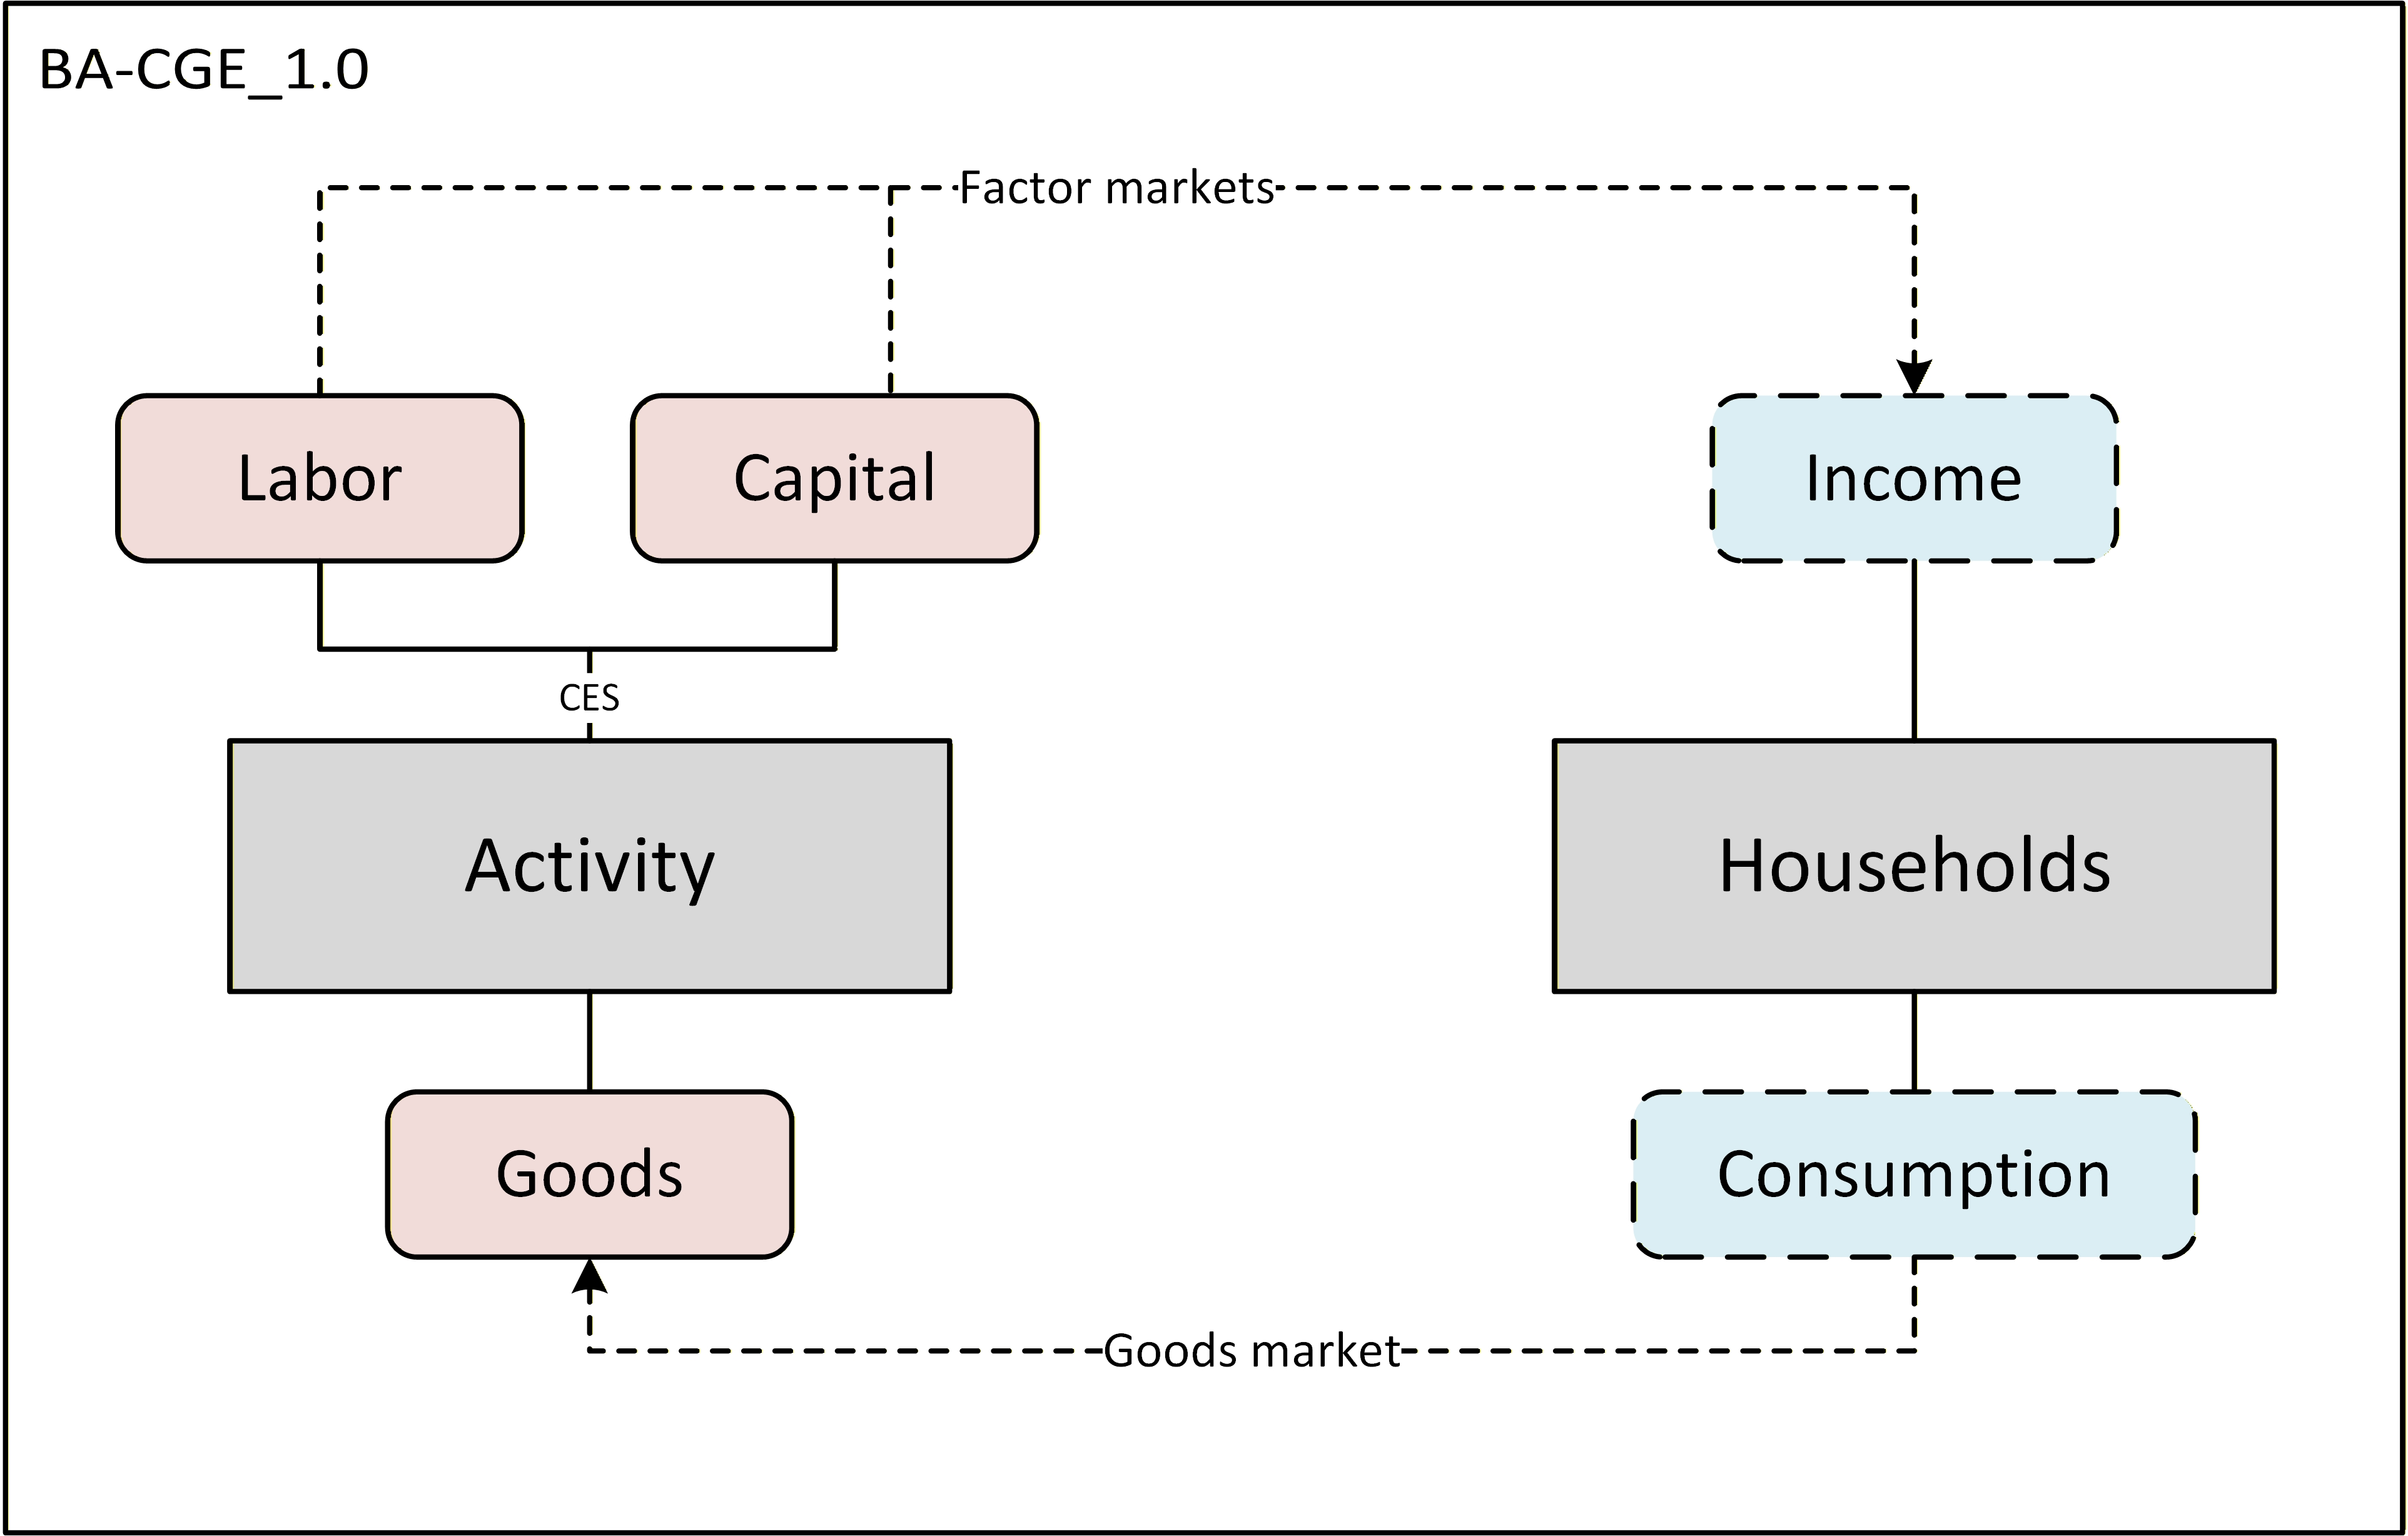
\includegraphics[width=\textwidth]{graphs/v1.0 structure.jpg}
	\caption{Model structure of BA-CGE v1.0}
	\label{v1.0-graph-structure}
\end{figure}

%1.2 Notations %%%%%%%%%%%%%%%%%%%%%%%%%%%%%%%%%%%%%%%%%%%%%%%%%%%%%
\subsection{Notations}\label{v1.0-notations}
See Tables \ref{v1.0-model-variables} -- \ref{v1.0-other-notations}.

\begin{table}[htbp]
	\centering
	\caption{Model variables}
	\label{v1.0-model-variables}
	\small
	\begin{tabularx}{\linewidth}{@{} l X @{}}
		\toprule
		\textbf{Variables} & \textbf{Descriptions} \\
		\midrule
		$L$	& Quantities of labor \\
		$K$	& Quantities of capital \\
		$Q$ 	& Quantities of goods \\
		$U$ 	& Values of households utility \\
		$Y$ 	& Values of households income \\
		$W$ 	& Price of labor (wages) \\
		$R$ 	& Price of capital (rents) \\
		$P$ 	& Price of goods \\
		$D$ 	& Dummy variable for Walras test \\
		\bottomrule
	\end{tabularx}
\end{table}

\begin{table}[htbp]
	\centering
	\caption{Model parameters}
	\label{v1.0-model-parameters}
	\small
	\begin{tabularx}{\linewidth}{@{} l X @{}}
		\toprule
		\textbf{Parameters} & \textbf{Descriptions} \\
		\midrule
		$\sigma$		& Substitution elasticity between labor and capital \\
		$\alpha_l$ 	& Cost share of labor in production function \\
		$\alpha_k$ 	& Cost share of capital in production function \\
		$a$        		& Total factor productivity in production function \\
		$\lambda_l$	& Labor-augmented technical shifter \\
		$\lambda_k$ 	& Capital-augmented technical shifter \\
		$\bar{L}$		& Exogenous labor endowment \\
		$\bar{K}$		& Exogenous capital endowment \\
		\bottomrule
	\end{tabularx}
\end{table}

\begin{table}[htbp]
	\centering
	\caption{Other notations}
	\label{v1.0-other-notations}
	\small
	\begin{tabularx}{\linewidth}{@{} l X @{}}
		\toprule
		\textbf{Parameters} & \textbf{Descriptions} \\
		\midrule
		$\Pi$	& Unit profit of production (the net difference between unit revenue and unit cost) \\
		\bottomrule
	\end{tabularx}
\end{table}

%1.3 Model equations %%%%%%%%%%%%%%%%%%%%%%%%%%%%%%%%%%%%%%%%%%%%%%%%%%%%%
\subsection{Model equations}\label{v1.0-equations}
\textbf{Production module:}
\begin{itemize}
	\item Intermediate calculation -- Conditional labor demand function (\(L\_eq\)): 
	\begin{equation}
		L = \frac{\partial\Pi}{\partial W}Q = \lambda_{l}^{\sigma-1}\alpha_{l}\left(\frac{P}{W}\right)^\sigma Q
	\end{equation}
	\item Intermediate calculation -- Conditional capital demand function (\(K\_eq\)): 
	\begin{equation}
		K = \frac{\partial\Pi}{\partial R}Q = \lambda_{k}^{\sigma-1}\alpha_{k}\left(\frac{P}{R}\right)^\sigma Q
	\end{equation}
	\item Zero-profit condition -- Goods output (\(Q\_eq\)): 
	\begin{equation}
		0\geq\Pi = 
		\begin{cases}
		 P-\left[\alpha_{l}\left(\frac{W}{\lambda_{l}}\right)^{1-\sigma}+\alpha_{k}\left(\frac{R}{\lambda_{k}}\right)^{1-\sigma}\right]^{\frac{1}{1-\sigma}},\; \sigma\ne1\\
		 P-\frac{1}{a}\left[\left(\frac{1}{\lambda_{l}}\frac{W}{\alpha_l}\right)^{\alpha_{l}}\left(\frac{1}{\lambda_{k}}\frac{R}{\alpha_k}\right)^{\alpha_{k}}\right],\; \sigma=1
		\end{cases}
		\;\perp\; Q
	\end{equation}
\end{itemize}

\textbf{Households module:} 
\begin{itemize}
	\item Indicator calculation -- Households utility function (\(U\_eq\)): 
	\begin{equation}
		U = lnQ
	\end{equation}
	\item Intermediate calculation -- Households income balance (\(Y\_eq\)): 
	 \begin{equation}
		Y = WL+RK
	\end{equation}
\end{itemize}

\textbf{Market clearance:}
\begin{itemize}
	\item Market clearance -- Labor (\(W\_eq\)): 
	\begin{equation}
		0\geq L-\bar{L}\; \perp\; W
	\end{equation}
	\item Market clearance -- Capital (\(R\_eq\)): 
	\begin{equation}
		0\geq K-\bar{K}\; \perp\; R
	\end{equation}
	\item Market clearance -- Goods (\(P\_eq\))\footnote{
	Note that this equation is dummied because \(P\) is set as the numeraire.}: 
	\begin{equation}
		D = \frac{Y}{P}-Q
	\end{equation}
\end{itemize}

%1.4 Extensions to v1.0 %%%%%%%%%%%%%%%%%%%%%%%%%%%%%%%%%%%%%%%%%%%%%%%%%%%%%
\subsection{Extensions to v1.0}\label{v1.0-extensions}
BA-CGE v1.1 adds households savings and investments into the model, 
and v1.2 adds government into the model. 
For these versions, refer to \textit{Model update log} document. 

\clearpage

%2 BA-CGE v2.0 %%%%%%%%%%%%%%%%%%%%%%%%%%%%%%%%%%%%%%%%%%%%%%%%%%%%%%%%%%%%%%%%%%%%%%%%%%%%%%
\section{BA-CGE v2.0} \label{BA-CGE v2.0}
This is a simple \textbf{single-region, single-sector, two-factor, open-economy} CGE model.
The firm maximizes its profit subjected to constant return-to-scale CES technology.
The households save a fixed proportion of its income into the bank,
and then maximize its utility (increasing and convex) subjected to the budget constraint.
The government levies a production tax, a direct tax and an import tariff, and uses its income to purchase.
It operates with a constant fiscal surplus by lending to/borrowing from the bank.
The investment bank absorbs households savings and government net surplus, and forms into investment.
Imports are specified using Armington assumption, while exports follow the CET function. 
In total, there are seven markets: five goods markets (activity output, exports, domestic goods, imports, composite goods) and two factor markets. 

%2.1 Structure %%%%%%%%%%%%%%%%%%%%%%%%%%%%%%%%%%%%%%%%%%%%%%%%%%%%%
\subsection{Structure}\label{v2.0-structure}
See Figure \ref{v2.0-graph-structure}. 
\begin{figure}[h]
	\centering
	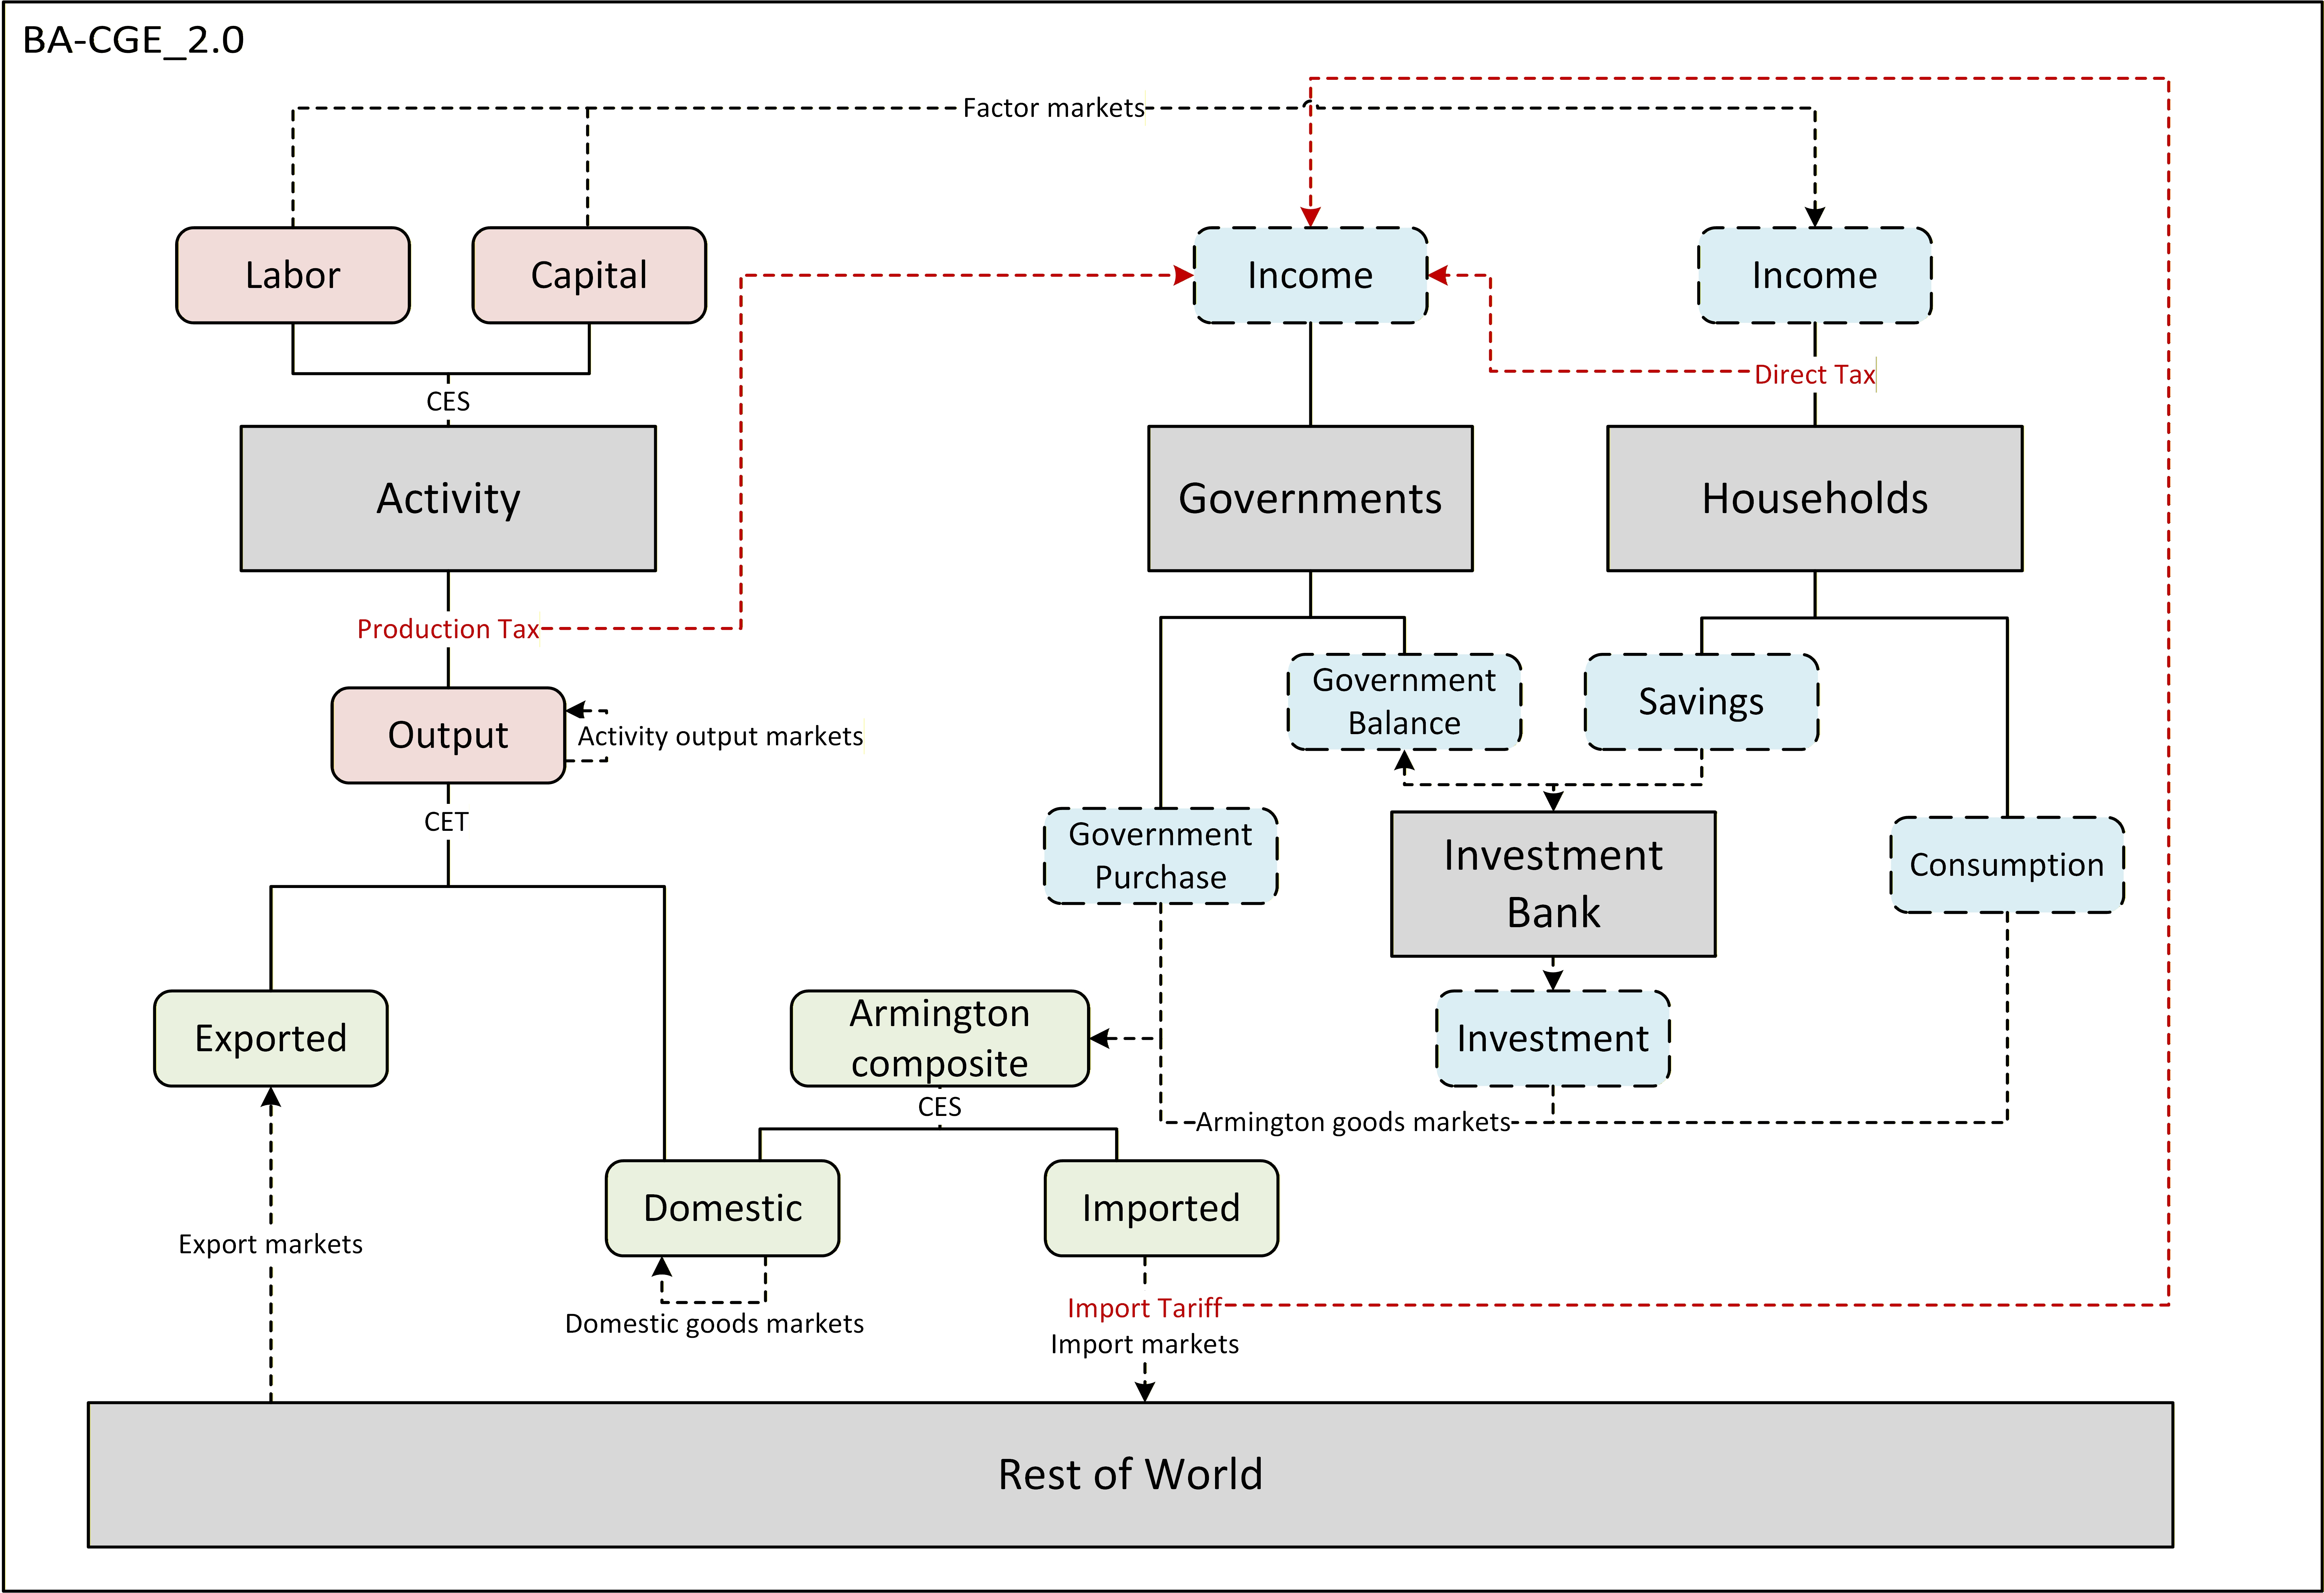
\includegraphics[width=\textwidth]{graphs/v2.0 structure.jpg}
	\caption{Model structure of BA-CGE v2.0}
	\label{v2.0-graph-structure}
\end{figure}

%1.2 Notations %%%%%%%%%%%%%%%%%%%%%%%%%%%%%%%%%%%%%%%%%%%%%%%%%%%%%
\subsection{Notations}\label{v2.0-notations}
See Tables \ref{v2.0-model-variables-prices} -- \ref{v2.0-other-notations}. 

\begin{table}[htbp]
	\centering
	\caption{Model variables -- Prices}
	\label{v2.0-model-variables-prices}
	\small
	\begin{tabularx}{\linewidth}{@{} l X @{}}
		\toprule
		\textbf{Variables} & \textbf{Descriptions} \\
		\midrule
		$P^{At}$	& Price of activity output (pre-tax) \\
		$P^{Mt}$	& Price of imported goods (pre-tax) \\
		$P^{P}$	& Price of households composite goods \\
		$P^{G}$	& Price of government composite goods \\
		$P^{I}$	& Price of investment composite goods \\
		$P^{L}$	& Price of labor (wages) \\
		$P^{K}$	& Price of capital (rents) \\
		$P^{A}$	& Price of activity output \\
		$P^{D}$	& Price of domestic goods \\
		$P^{E}$	& Price of exported goods \\
		$P^{M}$	& Price of imported goods \\
		$P^{C}$	& Price of composite goods \\
		\bottomrule
	\end{tabularx}
\end{table}

\begin{table}[htbp]
	\centering
	\caption{Model variables -- Quantities}
	\label{v2.0-model-variables-quantities}
	\small
	\begin{tabularx}{\linewidth}{@{} l X @{}}
		\toprule
		\textbf{Variables} & \textbf{Descriptions} \\
		\midrule
		$Q^{L}$	& Quantities of labor demand \\
		$Q^{K}$	& Quantities of capital demand \\
		$Q^{A}$	& Quantities of activity output supply \\
		$Q^{D}$	& Quantities of domestic goods supply \\
		$Q^{E}$	& Quantities of exported goods supply \\
		$Q^{M}$	& Quantities of imported goods demand \\
		$Q^C$	& Quantities of composite goods supply \\
		$Q^P$	& Quantities of households composite goods \\
		$Q^G$	& Quantities of government composite goods \\
		$Q^I$	& Quantities of investment composite goods \\
		\bottomrule
	\end{tabularx}
\end{table}

\begin{table}[htbp]
	\centering
	\caption{Model variables -- Values and others}
	\label{v2.0-model-variables-values}
	\small
	\begin{tabularx}{\linewidth}{@{} l X @{}}
		\toprule
		\textbf{Variables} & \textbf{Descriptions} \\
		\midrule
		$S^F$	& Values of net foreign savings \\
		$C^P$	& Values of households consumption \\
		$S^P$	& Values of households savings \\
		$Y^P$	& Values of households income\\
		$C^G$	& Values of government purchase\\
		$S^G$	& Values of government fiscal surplus\\
		$Y^G$	& Values of government income\\
		$Y^I$	& Values of investment expenditures\\
		$D$ 		& Dummy variable for Walras test \\
		\bottomrule
	\end{tabularx}
\end{table}

\begin{table}[htbp]
	\centering
	\caption{Model parameters -- Elasticities}
	\label{v2.0-model-parameters-elasticites}
	\small
	\begin{tabularx}{\linewidth}{@{} l X @{}}
		\toprule
		\textbf{Parameters} & \textbf{Descriptions} \\
		\midrule
		$\sigma^t$	& Substitution elasticity between labor and capital \\
		$\omega^x$	& Transformation elasticity between domestic and exported goods \\
		$\sigma^m$	& Substitution elasticity between domestic and imported goods \\
		\bottomrule
	\end{tabularx}
\end{table}

\begin{table}[htbp]
	\centering
	\caption{Model parameters -- Structures}
	\label{v2.0-model-parameters-structures}
	\small
	\begin{tabularx}{\linewidth}{@{} l X @{}}
		\toprule
		\textbf{Parameters} & \textbf{Descriptions} \\
		\midrule
		$\alpha_l$ 	& Cost share of labor in production function \\
		$\alpha_k$ 	& Cost share of capital in production function \\
		$a_a$        	& Scale parameter in production function \\
		$\lambda_l$	& Labor-augmented technical shifter \\
		$\lambda_k$ 	& Capital-augmented technical shifter \\
		$\gamma_d$ 	& Cost share of domestic goods in export CET function \\
		$\gamma_e$ 	& Cost share of exported goods in export CET function \\
		$\alpha_d$ 	& Cost share of domestic goods in armington import nest function \\
		$\alpha_m$ 	& Cost share of imported goods in armington import nest function \\
		$a_m$        	& Scale parameter in armington import nest function \\
		$\tau^p$	& Tax rate on production \\
		$\tau^m$	& Tax rate on imports \\
		$\beta^s$	& Households saving propensity \\
		$\tau^h$	& Tax rate on households income \\
		\bottomrule
	\end{tabularx}
\end{table}

\begin{table}[htbp]
	\centering
	\caption{Model parameters -- Closures}
	\label{v2.0-model-parameters-closures}
	\small
	\begin{tabularx}{\linewidth}{@{} l X @{}}
		\toprule
		\textbf{Parameters} & \textbf{Descriptions} \\
		\midrule
		$\overline{S}^G$ 	& Exogenous real government savings \\
		$\overline{Q}^L$	& Exogenous labor supply \\
		$\overline{Q}^K$	& Exogenous capital supply \\
		$\overline{Q}^E$	& Exogenous export demand \\
		$\overline{p}^{Ew}$	& Fixed world price of exported goods \\
		$\overline{p}^{Mw}$	& Fixed world price of imported goods \\
		\bottomrule
	\end{tabularx}
\end{table}

\begin{table}[htbp]
	\centering
	\caption{Other notations}
	\label{v2.0-other-notations}
	\small
	\begin{tabularx}{\linewidth}{@{} l X @{}}
		\toprule
		\textbf{Parameters} & \textbf{Descriptions} \\
		\midrule
		$\Pi^A$	& Unit profit of production (the net difference between unit revenue and unit cost) \\
		$\Pi^E$	& Unit profit of export CET \\
		$\Pi^C$	& Unit profit of Armington composite \\
		$\Pi^P$	& Unit profit of households composite \\
		$\Pi^G$	& Unit profit of government composite \\
		$\Pi^I$	& Unit profit of investment composite \\
		$GDP$	& Gross domestic production \\
		\bottomrule
	\end{tabularx}
\end{table}

%1.3 Model equations %%%%%%%%%%%%%%%%%%%%%%%%%%%%%%%%%%%%%%%%%%%%%%%%%%%%%
\subsection{Model equations}\label{v2.0-equations}
\textbf{Production module:}
\begin{itemize}
	\item Intermediate calculation -- Conditional demand function of labor (\(QL\_eq\)): 
	\begin{equation}
		Q^L = \frac{\partial\Pi^A}{\partial P^L}Q^A = \lambda_{l}^{\sigma^t-1}\alpha_{l}\left(\frac{P^{At}}{P^L}\right)^{\sigma^{t}}Q^A
	\end{equation}
	\item Intermediate calculation -- Conditional demand function of capital (\(QK\_eq\)): 
	\begin{equation}
		Q^K = \frac{\partial\Pi^A}{\partial P^K}Q^A = \lambda_{k}^{\sigma^t-1}\alpha_{k}\left(\frac{P^{At}}{P^K}\right)^{\sigma^{t}}Q^A
	\end{equation}
	\item Zero-profit condition -- Activity output (supply) (\(QA\_eq\)): 
	\begin{equation}
		0\geq\Pi^A = 
		\begin{cases}
		 P^{At}-\left[\alpha_{l}\left(\frac{P^L}{\lambda_{l}}\right)^{1-\sigma^t}+\alpha_{k}\left(\frac{P^K}{\lambda_{k}}\right)^{1-\sigma^t}\right]^{\frac{1}{1-\sigma^t}},\; \sigma^t\ne1\\
		 P^{At}-\frac{1}{a_a}\left[\left(\frac{1}{\lambda_{l}}\frac{P^L}{\alpha_l}\right)^{\alpha_{l}}\left(\frac{1}{\lambda_{k}}\frac{P^K}{\alpha_k}\right)^{\alpha_{k}}\right],\; \sigma^t=1
		\end{cases}
		\;\perp\; Q^A
	\end{equation}
	\item Intermediate calculation -- Calculation of pre-tax price (production tax) (\(PAT\_eq\)): 
	\begin{equation}
		P^{At} = \frac{P^A}{1+\tau^p}
	\end{equation}
\end{itemize}

\textbf{Trade module:}
\begin{itemize}
	\item Intermediate calculation -- Conditional supply function of domestic goods (\(QD\_eq\))\footnote{
	Note that when \(\omega^x=\infty\), the supply of domestic goods is governed by law-of-one-price. 
	Similar expressions apply here-in-after.}: 
	\begin{equation}
		\begin{cases}
		Q^D = \frac{\partial\Pi^E}{\partial P^D}Q^A = \gamma_{d}\left(\frac{P^D}{P^A}\right)^{\omega^{x}}Q^A, \; \omega^x\ne\infty\\
		P^D = P^A, \; \omega^x=\infty
		\end{cases}
	\end{equation}
	\item Intermediate calculation -- Conditional supply function of exported goods (\(QE\_eq\)): 
	\begin{equation}
		\begin{cases}
		Q^E = \frac{\partial\Pi^E}{\partial P^E}Q^A = \gamma_{e}\left(\frac{P^E}{P^A}\right)^{\omega^{x}}Q^A, \; \omega^x\ne\infty\\
		P^E = P^A, \; \omega^x=\infty
		\end{cases}
	\end{equation}
	\item Zero-profit condition -- Activity output (demand) (\(QA\_eq\))\footnote{
	Note that this equation is omitted and is essentially substituted by the market clearance PA\_eq.}: 
	\begin{equation}
		0\geq
		\begin{cases}
		 \Pi^E = \left(\gamma_{d}{P^D}^{1+\omega^x}+\gamma_{e}{P^E}^{1+\omega^x}\right)^{\frac{1}{1+\omega^x}} - P^A,\; \omega^x\ne\infty\\
		 \left(Q^D+Q^E\right) - Q^A,\; \omega^x=\infty
		\end{cases}
		\;\perp\; Q^A
	\end{equation}
	\item Intermediate calculation -- Calculation of pre-tax price (import tariff) (\(PMT\_eq\)): 
	\begin{equation}
		P^{Mt} = \frac{P^M}{1+\tau^m}
	\end{equation}
	\item Intermediate calculation -- Conditional demand function of domestic goods (\(QD\_eq\))\footnote{
	Note that this equation is omitted and is essentially substituted by the market clearance PD\_eq.}: 
	\begin{equation}
		Q^D = \frac{\partial\Pi^C}{\partial P^D}Q^C = \alpha_{d}\left(\frac{P^C}{P^D}\right)^{\sigma^{m}}Q^C
	\end{equation}
	\item Intermediate calculation -- Conditional demand function of imported goods (\(QM\_eq\)): 
	\begin{equation}
		Q^M = \frac{\partial\Pi^C}{\partial P^M}Q^C = \alpha_{m}\left(\frac{P^C}{P^M}\right)^{\sigma^{m}}Q^C
	\end{equation}
	\item Zero-profit condition -- Composite goods (\(QC\_eq\)): 
	\begin{equation}
		0\geq\Pi^C = 
		\begin{cases}
		 P^C-\left(\alpha_{d}{P^D}^{1-\sigma^m}+\alpha_{m}{P^M}^{1-\sigma^m}\right)^{\frac{1}{1-\sigma^m}},\; \sigma^m\ne1\\
		 P^C-\frac{1}{a_m}\left[\left(\frac{P^D}{\alpha_{d}}\right)^{\alpha_{d}}\left(\frac{P^M}{\alpha_{m}}\right)^{\alpha_{m}}\right],\; \sigma^m=1
		\end{cases}
		\;\perp\; Q^C
	\end{equation}
	\item Intermediate calculation -- Calculation of net foreign savings (\(YFS\_eq\)): 
	\begin{equation}
		S^F = P^{Mt}Q^{M} - P^{E}Q^{E}
	\end{equation}
\end{itemize}

\textbf{Households module:}
\begin{itemize}
	\item Zero-profit condition -- Households composite goods (\(QP\_eq\)): 
	\begin{equation}
		0\geq\Pi^P = P^P - P^C \;\perp\; Q^P
	\end{equation}
	\item Market clearance -- Households composite goods (\(PP\_eq\)): 
	\begin{equation}
		0\geq C^P - P^{P}Q^{P} \;\perp\; P^P
	\end{equation}
	\item Intermediate calculation -- Calculation of households consumption (\(YPC\_eq\)): 
	\begin{equation}
		C^P = \left(1-\beta^s\right)Y^P
	\end{equation}
	\item Intermediate calculation -- Calculation of households savings (\(YPS\_eq\)): 
	\begin{equation}
		S^P = \beta^{s}Y^P
	\end{equation}
	\item Intermediate calculation -- Households income balance (\(YP\_eq\)): 
	\begin{equation}
		Y^P = \left(1-\tau^h\right)\left(P^{L}Q^{L} + P^{K}Q^{K}\right)
	\end{equation}
\end{itemize}

\textbf{Government module:}
\begin{itemize}
	\item Zero-profit condition -- Government composite goods (\(QG\_eq\)): 
	\begin{equation}
		0\geq\Pi^G = P^G - P^C \;\perp\; Q^G
	\end{equation}
	\item Market clearance -- Government composite goods (\(PG\_eq\)): 
	\begin{equation}
		0\geq C^G - P^{G}Q^{G} \;\perp\; P^G
	\end{equation}
	\item Intermediate calculation -- Calculation of government consumption (\(YGC\_eq\)): 
	\begin{equation}
		C^G = Y^G - S^G
	\end{equation}
	\item Intermediate calculation -- Calculation of government savings (\(YGS\_eq\)): 
	\begin{equation}
		S^G = \overline{S}^{G}P^{G}
	\end{equation}
	\item Intermediate calculation -- Government income balance (\(YG\_eq\)): 
	\begin{equation}
		Y^G = \tau^{p}Q^{A}P^{At} + \tau^{m}Q^{M}P^{Mt} + \tau^{h}\left(P^{L}Q^{L} + P^{K}Q^{K}\right)
	\end{equation}
\end{itemize}

\textbf{Investment module:}
\begin{itemize}
	\item Zero-profit condition -- Investment composite goods (\(QI\_eq\)): 
	\begin{equation}
		0\geq\Pi^I = P^I - P^C \;\perp\; Q^I
	\end{equation}
	\item Market clearance -- Investment composite goods (\(PI\_eq\)): 
	\begin{equation}
		0\geq Y^I - P^{I}Q^{I} \;\perp\; P^I
	\end{equation}
	\item Intermediate calculation -- Savings-investment balance (\(YI\_eq\)): 
	\begin{equation}
		Y^I = S^P+S^G+S^F
	\end{equation}
\end{itemize}

\textbf{Market Clearance:}
\begin{itemize}
	\item Market clearance -- Labor (\(PL\_eq\)): 
	\begin{equation}
		0\geq Q^L - \overline{Q}^L \;\perp\; P^L
	\end{equation}
	\item Market clearance -- Capital (\(PK\_eq\)): 
	\begin{equation}
		0\geq Q^K - \overline{Q}^K \;\perp\; P^K
	\end{equation}
	\item Market clearance -- Activity output (\(PA\_eq\)): 
	\begin{equation}
		0\geq Q^{A}(d) - Q^{A}(s)
		\;\perp\; P^A
	\end{equation}
	\item Market clearance -- Domestic goods (\(PD\_eq\)): 
	\begin{equation}
		0\geq Q^{D}(d) - Q^{D}(s)
		\;\perp\; P^D
	\end{equation}
	\item Market clearance -- Exported goods (\(PE\_eq\)): 
	\begin{equation}
		0 = 
		\begin{cases}
			P^E - \overline{p}^{Ew}P^C\\
			Q^E - \overline{Q}^E
		\end{cases}
		\;\perp\; P^E
	\end{equation}
	\item Market clearance -- Imported goods (\(PM\_eq\)): 
	\begin{equation}
		0 = P^{Mt} - \overline{p}^{Mw}P^C
		\;\perp\; P^M
	\end{equation}
	\item Market clearance -- Composite goods (\(PC\_eq\))\footnote{
	Note that this equation is dummied because \(PC\) is set as the numeraire.}: 
	\begin{equation}
		D = \left(Q^P+Q^G+Q^I\right) - Q^C
	\end{equation}
\end{itemize}

\textbf{Indices:}
\begin{itemize}
	\item Indicator calculation -- GDP (\(GDP\_eq\)): 
	\begin{equation}
		GDP = P^{P}Q^{P}+P^{G}Q^{G}+P^{I}Q^{I}+P^{E}Q^{E}-P^{Mt}Q^{M}
	\end{equation}
\end{itemize}































\end{document}